%%%%%%%%%%%%%%%%%%%%%%%%%%%%%%%%%%%%%%%%%%%%%%%%%%%%%%%%%%%%%%%%%%%%%%%%%%%%%%%%%%%%%%%%%%%%%%%%%%%%%%%%%%%%%%%%%%%%%%%%%
\subsection{Synergies}
%%%%%%%%%%%%%%%%%%%%%%%%%%%%%%%%%%%%%%%%%%%%%%%%%%%%%%%%%%%%%%%%%%%%%%%%%%%%%%%%%%%%%%%%%%%%%%%%%%%%%%%%%%%%%%%%%%%%%%%%%

\begin{frame}{Synergies}
    \begin{itemize}
        \item \textbf{Reinforcement Learning}: Learning to achieve a goal with interventions.
        \item \textbf{Causal Learning}: Learning how the world works with interventions.
    \end{itemize}

    \pause
    \vspace{1cm}
    It looks like both of these learning methodologies revolve around \textbf{interventional data}.

    Additionally, learning a more descriptive representation of the world (through causal learning) can help
    Reinforcement Learning.
\end{frame}
%%%%%%%%%%%%%%%%%%%%%%%%%%%%%%%%%%%%%%%%%%%%%%%%%%%%%%%%%%%%%%%%%%%%%%%%%%%%%%%%%%%%%%%%%%%%%%%%%%%%%%%%%%%%%%%%%%%%%%%%%
\subsection{The Field}
%%%%%%%%%%%%%%%%%%%%%%%%%%%%%%%%%%%%%%%%%%%%%%%%%%%%%%%%%%%%%%%%%%%%%%%%%%%%%%%%%%%%%%%%%%%%%%%%%%%%%%%%%%%%%%%%%%%%%%%%%

\begin{frame}{The Field}
    The idea of joining Causality with Reinforcement Learning 
    is called recently began to be explored and is called \textbf{Causal Reinforcement Learning}.

    \begin{figure}[l]
        \centering
        \vspace{0pt}
        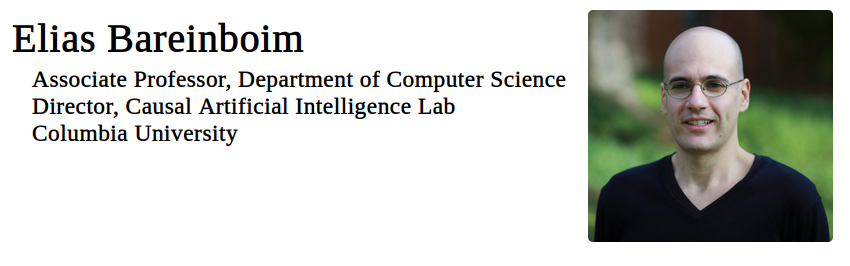
\includegraphics[width=0.7\textwidth]{img/elias.png}
    \end{figure}

    \footnotetext[3]{Source: \url{https://causalai.net/}}

\end{frame}